% Created 2021-05-31 Mon 15:41
% Intended LaTeX compiler: pdflatex
\documentclass[11pt]{article}
\usepackage[utf8]{inputenc}
\usepackage[T1]{fontenc}
\usepackage{graphicx}
\usepackage{grffile}
\usepackage{longtable}
\usepackage{wrapfig}
\usepackage{rotating}
\usepackage[normalem]{ulem}
\usepackage{amsmath}
\usepackage{textcomp}
\usepackage{amssymb}
\usepackage{capt-of}
\usepackage{hyperref}
% \usepackage{amsmath}
\date{\today}
\title{}
\hypersetup{
 pdfauthor={},
 pdftitle={},
 pdfkeywords={},
 pdfsubject={},
 pdfcreator={Emacs 27.2 (Org mode 9.4.6)}, 
 pdflang={English}}
\usepackage{graphicx}
\graphicspath{{./img-plots/}
  {./}}

\begin{document}

\tableofcontents

Medir a indução magnética do material vs campo magnético aplicado

\(B = \mu_{0} H + \mu_{0} M\) 
\(M = \chi H\)

\begin{itemize}
\item Medida de Indução Magnética (\(M\))
\begin{itemize}
\item Fluxômetro ou fluxímetro.
\end{itemize}

\item Geração de Campo Magnético (H)
\begin{itemize}
\item Fonte de corrente.
\item Bobina grande de cobre.
\item Núcleo de Fe-Si em forma de U.
\end{itemize}
\end{itemize}


\section{Resultados}
\label{sec:org44cb2ec}
\subsection{Experimento 1  - Bobina primária, sem núcleo}
\label{sec:org4ef7571}
Por breviedade e concisão, apresentaremos os gráficos, em escala, justapostos das grandezas físicas plotadas contra o tempo.


\subsubsection{Análise gráfica}
\label{sec:orgd406928}

{\begin{figure}[htbp]

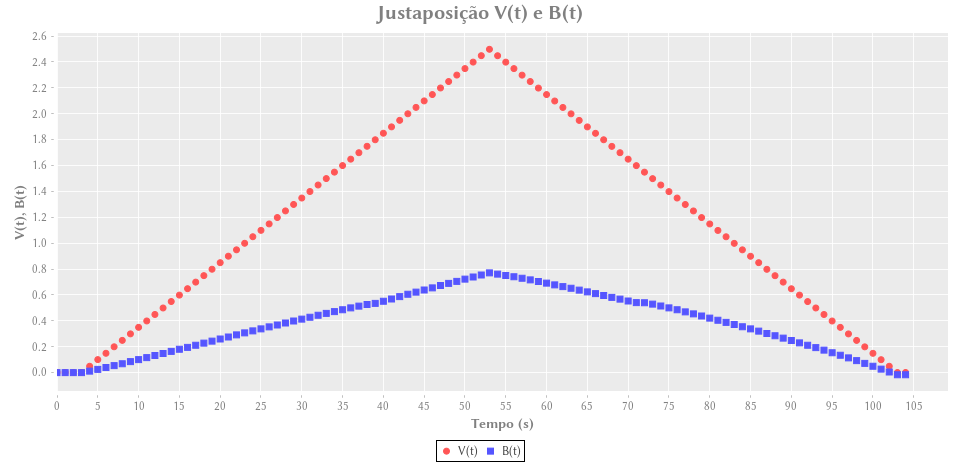
\includegraphics[width=.9\linewidth]{img-plots/V-B-justaposicao-sem-nucleo.png}
\caption{V(t) vs B(t), sem núcleo}
\end{figure}}

Existe uma proporcionalidade linearmente depente entre as curvas. Ou seja, para qualquer valor de V(t), B(t) corresponde a multiplicação de uma constate vezes V(t). O qual caracteriza \(B(t) \propto V(t)\), e.i., uma relação de proporções.

\subsection{Experimento 2 - Com núcleo, liga Fe-Si}
\label{sec:org8be7789}

\subsubsection{Análise gráfica}
\label{sec:org183bc3b}
{\begin{figure}[htbp]

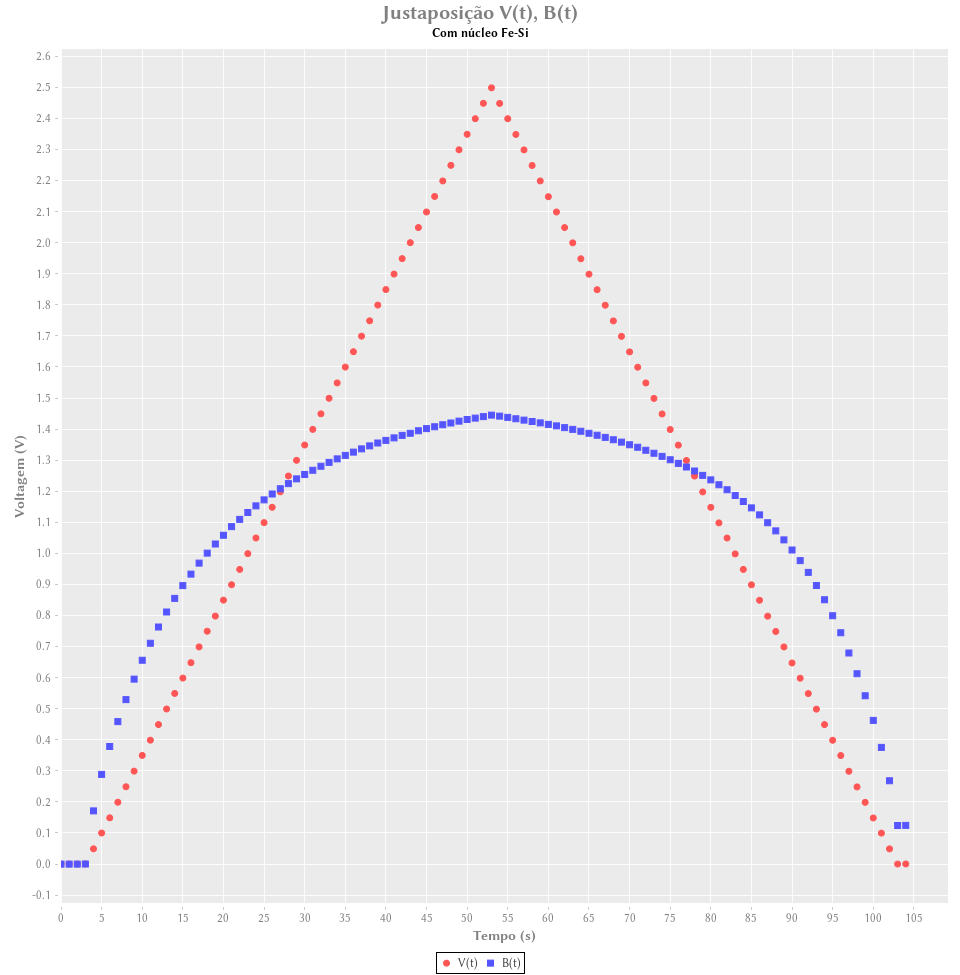
\includegraphics[width=.9\linewidth]{img-plots/V-B-justaposicao-com-nucleo.png}
\caption{V(t) vs B(t), meio de Fe-Si}
\end{figure}}

Com Fe-Si, as curvas continuam isomórficas. Isto é, para qualquer par \((t_1, t_2)\), e qualquer par das funções \((V(t),B(t))\), a relação isomórfica \cite{pinter2014book} é satisfeita,

\begin{equation}
   V(t_1) < V(t_2) \Leftrightarrow B(t_1) < B(t_2)
\end{equation}

Porém, a relação não é mais linearmente proporcional.  Não existe uma constate que possa ser atribuida a relação de proporção entre V e B. Ademais, há um nível de saturação em \(B\), em \(\approx 52,5 \, \textrm{segundos}\), no valor de \(2,5 V\). Nos intervalos simétricos de \([0, 1.2] V\), em relação ao tempo, existe um aumento de campo em relação ao caso com meio material Ar, \hyperref[sec:org4ef7571]{Bobina sem núcleo Fe-Si.}

\subsection{Experimento 3 - Histerese, liga Fe-Si}
\label{sec:org30e28f0}

\subsubsection{Análise Gráfica}
\label{sec:org34a6338}
{\begin{figure}[htbp]

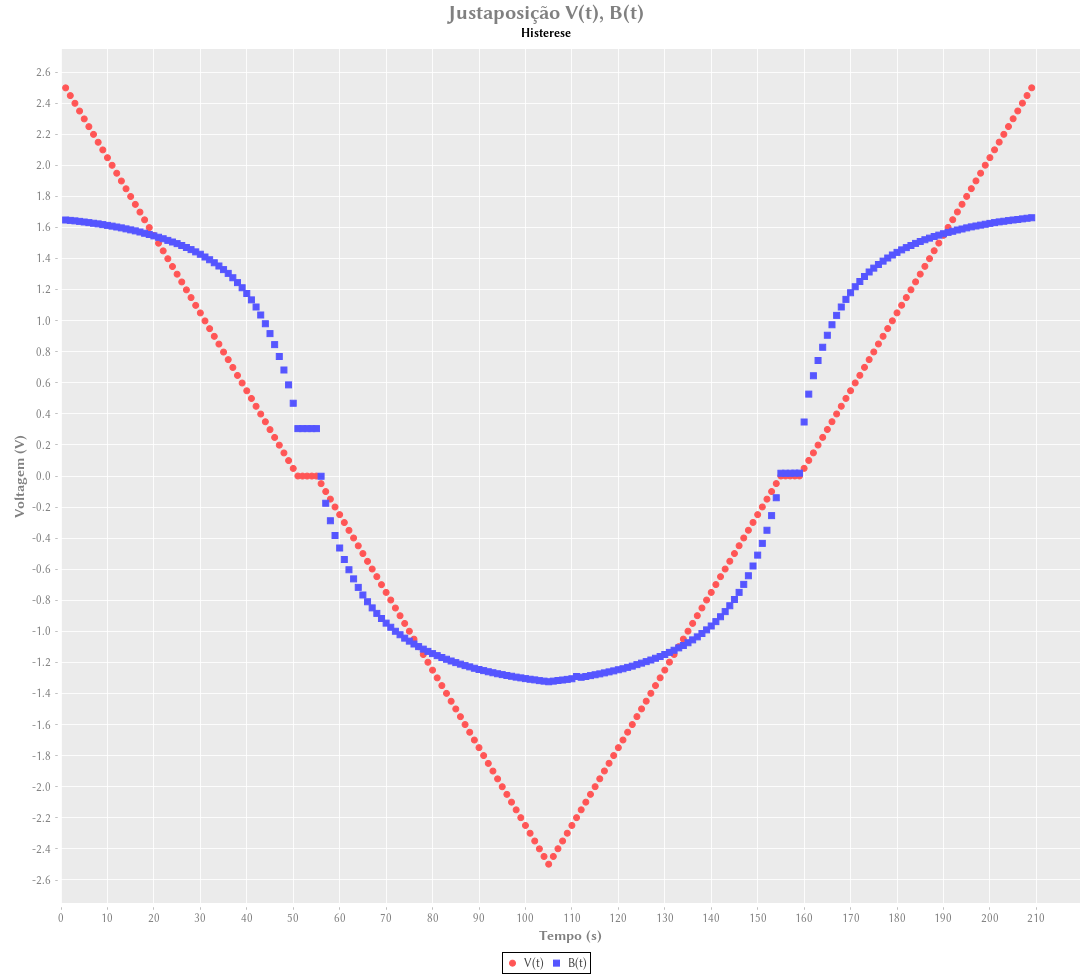
\includegraphics[width=.9\linewidth]{img-plots/V-B-justaposicao-histerese.png}
\caption{Histerese Fe-Si}
\end{figure}}

No caso de Histerese, também observamos a relação de  isomorfismo sendo preservado. Em especial, entre os valores não oscilantes de V, em \((t \, \epsilon \, [50, 60.5] \textrm{segundos}) \, \land (t \, \epsilon \, [150.5, 160] \textrm{segundos})\), observamos perfeitamente uma não-oscilação de B(t).


\subsection{Comparação ao caso sem e com material}
\label{sec:org3054bfb}
{\begin{figure}[htbp]

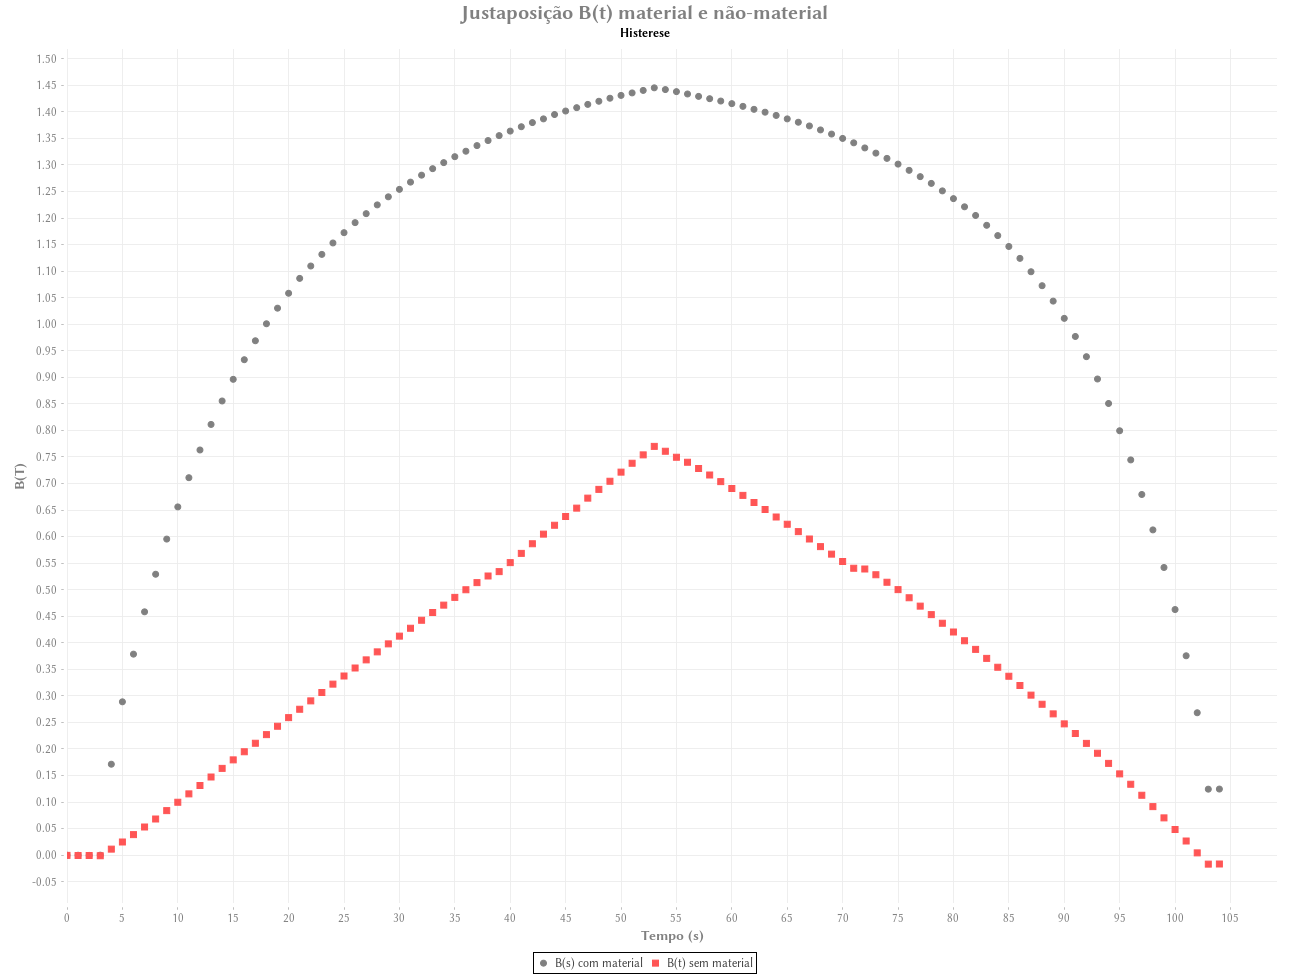
\includegraphics[width=.9\linewidth]{img-plots/B-justaposicao.png}
\caption{Superposição de B(t).}
\end{figure}}

Para qualquer valor de B(t), em qualque t no intervalo, a relação \(B_{\textrm{material}}(t)>B_{\textrm{sem-material}}(t)\) é verdadeira.

\section{Discussão}
\label{sec:orgeaf30e7}

\subsection{Diferenças entre os casos sem e com meio material}
\label{sec:orgd724b12}
Em ambos cenários  com e sem materiais existe uma relação isomórfica entre o campo aplicado \(V\) e \(B\). No entanto, particularmente, no caso em que essa relação é observada em um meio não-material como o Ar, a relação é linearmente depente, com o fator de proporção sendo uma constante. e.i., os gráficos são matematicamente \emph{semelhantes}.

Quando adicionamos um corpo material metálico, Fe-Si - o qual reage à diferença de potencial V, e campos elétromagnético, de forma não linear - a relação de isomorfismo é preservada. Assim, demonstrando que o material apenas reage ao campo V, aumentando ou diminuindo a relação de proporção, em diferentes níveis de excitações de campo e consequentes diferentes estados físicos de excitação. E, não existe nenhum outro fator externo o afetando, e.g., gravidade, temperatura, etc. Em particular, essa inexistência de variação decorrente de outros fatore é visível em \hyperref[sec:org34a6338]{Análise Gráfica - histerese}.

Em voltagens entre \([0, \pm 1.2]V\) o material de Fe-Si possui baixa saturação, e assim, acresce ao valor do campo, em comparação ao caso sem núcleo. Em voltagens maiores, em módulo, do que \(1.2V\) é atingida saturação de excitação do material, e consequentementes, há um fatos de decrescimento da taxa de aumento do campo \(B\), por aumento da tensão \(V\).

\subsection{Caso com material e a Histerese}
\label{sec:org7fd1a0b}

Os sub-experimentos 2 e 3 são, na verdade, experimentos em que o 2 é caso particular de 3. No gráfico da Histerese, os valores percorridos nos intervalos \((t \, \epsilon \, [0, 60] \textrm{segundos}) \, \land (t \, \epsilon \, [160, 220] \textrm{segundos})\) são exatamente os mesmos no sub-experimento 2, no intevalos correspondentes de \(t \, \epsilon \, [52.5, 105] \textrm{segundos} \land t \, \epsilon \, [0, 52.5] \textrm{segundos}\).
\end{document}